%%%%%%%%%%%%%%%%%%%%%%%%%%%%%%%%%%%%%%%%%
% Arsclassica Article
% LaTeX Template
% Version 1.1 (10/6/14)
%
% This template has been downloaded from:
% http://www.LaTeXTemplates.com
%
% Original author:
% Lorenzo Pantieri (http://www.lorenzopantieri.net) with extensive modifications by:
% Vel (vel@latextemplates.com)
%
% License:
% CC BY-NC-SA 3.0 (http://creativecommons.org/licenses/by-nc-sa/3.0/)
%
%%%%%%%%%%%%%%%%%%%%%%%%%%%%%%%%%%%%%%%%%

%----------------------------------------------------------------------------------------
%	PACKAGES AND OTHER DOCUMENT CONFIGURATIONS
%----------------------------------------------------------------------------------------

\documentclass[
10pt, % Main document font size
a4paper, % Paper type, use 'letterpaper' for US Letter paper
oneside, % One page layout (no page indentation)
%twoside, % Two page layout (page indentation for binding and different headers)
headinclude,footinclude, % Extra spacing for the header and footer
BCOR5mm, % Binding correction
]{scrartcl}

%%%%%%%%%%%%%%%%%%%%%%%%%%%%%%%%%%%%%%%%%
% Arsclassica Article
% Structure Specification File
%
% This file has been downloaded from:
% http://www.LaTeXTemplates.com
%
% Original author:
% Lorenzo Pantieri (http://www.lorenzopantieri.net) with extensive modifications by:
% Vel (vel@latextemplates.com)
%
% License:
% CC BY-NC-SA 3.0 (http://creativecommons.org/licenses/by-nc-sa/3.0/)
%
%%%%%%%%%%%%%%%%%%%%%%%%%%%%%%%%%%%%%%%%%

%----------------------------------------------------------------------------------------
%	REQUIRED PACKAGES
%----------------------------------------------------------------------------------------

\usepackage[
nochapters, % Turn off chapters since this is an article        
beramono, % Use the Bera Mono font for monospaced text (\texttt)
eulermath,% Use the Euler font for mathematics
pdfspacing, % Makes use of pdftex’ letter spacing capabilities via the microtype package
dottedtoc % Dotted lines leading to the page numbers in the table of contents
]{classicthesis} % The layout is based on the Classic Thesis style

\usepackage{arsclassica} % Modifies the Classic Thesis package

\usepackage[T1]{fontenc} % Use 8-bit encoding that has 256 glyphs

\usepackage[utf8]{inputenc} % Required for including letters with accents

\usepackage{graphicx} % Required for including images
\graphicspath{{Figures/}} % Set the default folder for images

\usepackage{enumitem} % Required for manipulating the whitespace between and within lists

\usepackage{lipsum} % Used for inserting dummy 'Lorem ipsum' text into the template

\usepackage{subfig} % Required for creating figures with multiple parts (subfigures)

\usepackage{amsmath,amssymb,amsthm} % For including math equations, theorems, symbols, etc

\usepackage{varioref} % More descriptive referencing
\usepackage{color}
\usepackage{listings}
\usepackage{setspace}

\usepackage{lscape}


%----------------------------------------------------------------------------------------
%	THEOREM STYLES
%---------------------------------------------------------------------------------------

\theoremstyle{definition} % Define theorem styles here based on the definition style (used for definitions and examples)
\newtheorem{definition}{Definition}

\theoremstyle{plain} % Define theorem styles here based on the plain style (used for theorems, lemmas, propositions)
\newtheorem{theorem}{Theorem}

\theoremstyle{remark} % Define theorem styles here based on the remark style (used for remarks and notes)

%----------------------------------------------------------------------------------------
%	HYPERLINKS
%---------------------------------------------------------------------------------------

\hypersetup{
%draft, % Uncomment to remove all links (useful for printing in black and white)
colorlinks=true, breaklinks=true, bookmarks=true,bookmarksnumbered,
urlcolor=webbrown, linkcolor=RoyalBlue, citecolor=webgreen, % Link colors
pdftitle={}, % PDF title
pdfauthor={\textcopyright}, % PDF Author
pdfsubject={}, % PDF Subject
pdfkeywords={}, % PDF Keywords
pdfcreator={pdfLaTeX}, % PDF Creator
pdfproducer={LaTeX with hyperref and ClassicThesis} % PDF producer
}

\definecolor{Code}{rgb}{0,0,0}
\definecolor{Decorators}{rgb}{0.5,0.5,0.5}
\definecolor{Numbers}{rgb}{0.5,0,0}
\definecolor{MatchingBrackets}{rgb}{0.25,0.5,0.5}
\definecolor{Keywords}{rgb}{0,0,1}
\definecolor{self}{rgb}{0,0,0}
\definecolor{Strings}{rgb}{0,0.63,0}
\definecolor{Comments}{rgb}{0,0.63,1}
\definecolor{Backquotes}{rgb}{0,0,0}
\definecolor{Classname}{rgb}{0,0,0}
\definecolor{FunctionName}{rgb}{0,0,0}
\definecolor{Operators}{rgb}{0,0,0}
\definecolor{Background}{rgb}{0.98,0.98,0.98}

\lstnewenvironment{python}[1][]{
\lstset{
numbers=left,
numberstyle=\footnotesize,
numbersep=1em,
xleftmargin=1em,
framextopmargin=2em,
framexbottommargin=2em,
showspaces=false,
showtabs=false,
showstringspaces=false,
frame=l,
tabsize=4,
% Basic
basicstyle=\ttfamily\small\setstretch{1},
backgroundcolor=\color{Background},
language=Python,
% Comments
commentstyle=\color{Comments}\slshape,
% Strings
stringstyle=\color{Strings},
morecomment=[s][\color{Strings}]{"""}{"""},
morecomment=[s][\color{Strings}]{'''}{'''},
% keywords
morekeywords={import,from,class,def,for,while,if,is,in,elif,else,not,and,or,print,break,continue,return,True,False,None,access,as,,del,except,exec,finally,global,import,lambda,pass,print,raise,try,assert},
keywordstyle={\color{Keywords}\bfseries},
% additional keywords
morekeywords={[2]@invariant},
keywordstyle={[2]\color{Decorators}\slshape},
emph={self},
emphstyle={\color{self}\slshape},
%
}}{}

 % Include the structure.tex file which specified the document structure and layout

\hyphenation{Fortran hy-phen-ation} % Specify custom hyphenation points in words with dashes where you would like hyphenation to occur, or alternatively, don't put any dashes in a word to stop hyphenation altogether

%----------------------------------------------------------------------------------------
%	TITLE AND AUTHOR(S)
%----------------------------------------------------------------------------------------

\title{\normalfont\spacedallcaps{Detecting local events in the Twitter stream}} % The article title

\author{\spacedlowsmallcaps{Chris Pool}} % The article author(s) - author affiliations need to be specified in the AUTHOR AFFILIATIONS block

\date{} % An optional date to appear under the author(s)

%----------------------------------------------------------------------------------------

\begin{document}

%----------------------------------------------------------------------------------------
%	HEADERS
%----------------------------------------------------------------------------------------

\renewcommand{\sectionmark}[1]{\markright{\spacedlowsmallcaps{#1}}} % The header for all pages (oneside) or for even pages (twoside)
%\renewcommand{\subsectionmark}[1]{\markright{\thesubsection~#1}} % Uncomment when using the twoside option - this modifies the header on odd pages
\lehead{\mbox{\llap{\small\thepage\kern1em\color{halfgray} \vline}\color{halfgray}\hspace{0.5em}\rightmark\hfil}} % The header style

\pagestyle{scrheadings} % Enable the headers specified in this block

%----------------------------------------------------------------------------------------
%	TABLE OF CONTENTS & LISTS OF FIGURES AND TABLES
%----------------------------------------------------------------------------------------

\maketitle % Print the title/author/date block
\begin{figure}[htbp] %  figure placement: here, top, bottom, or page
   \centering
   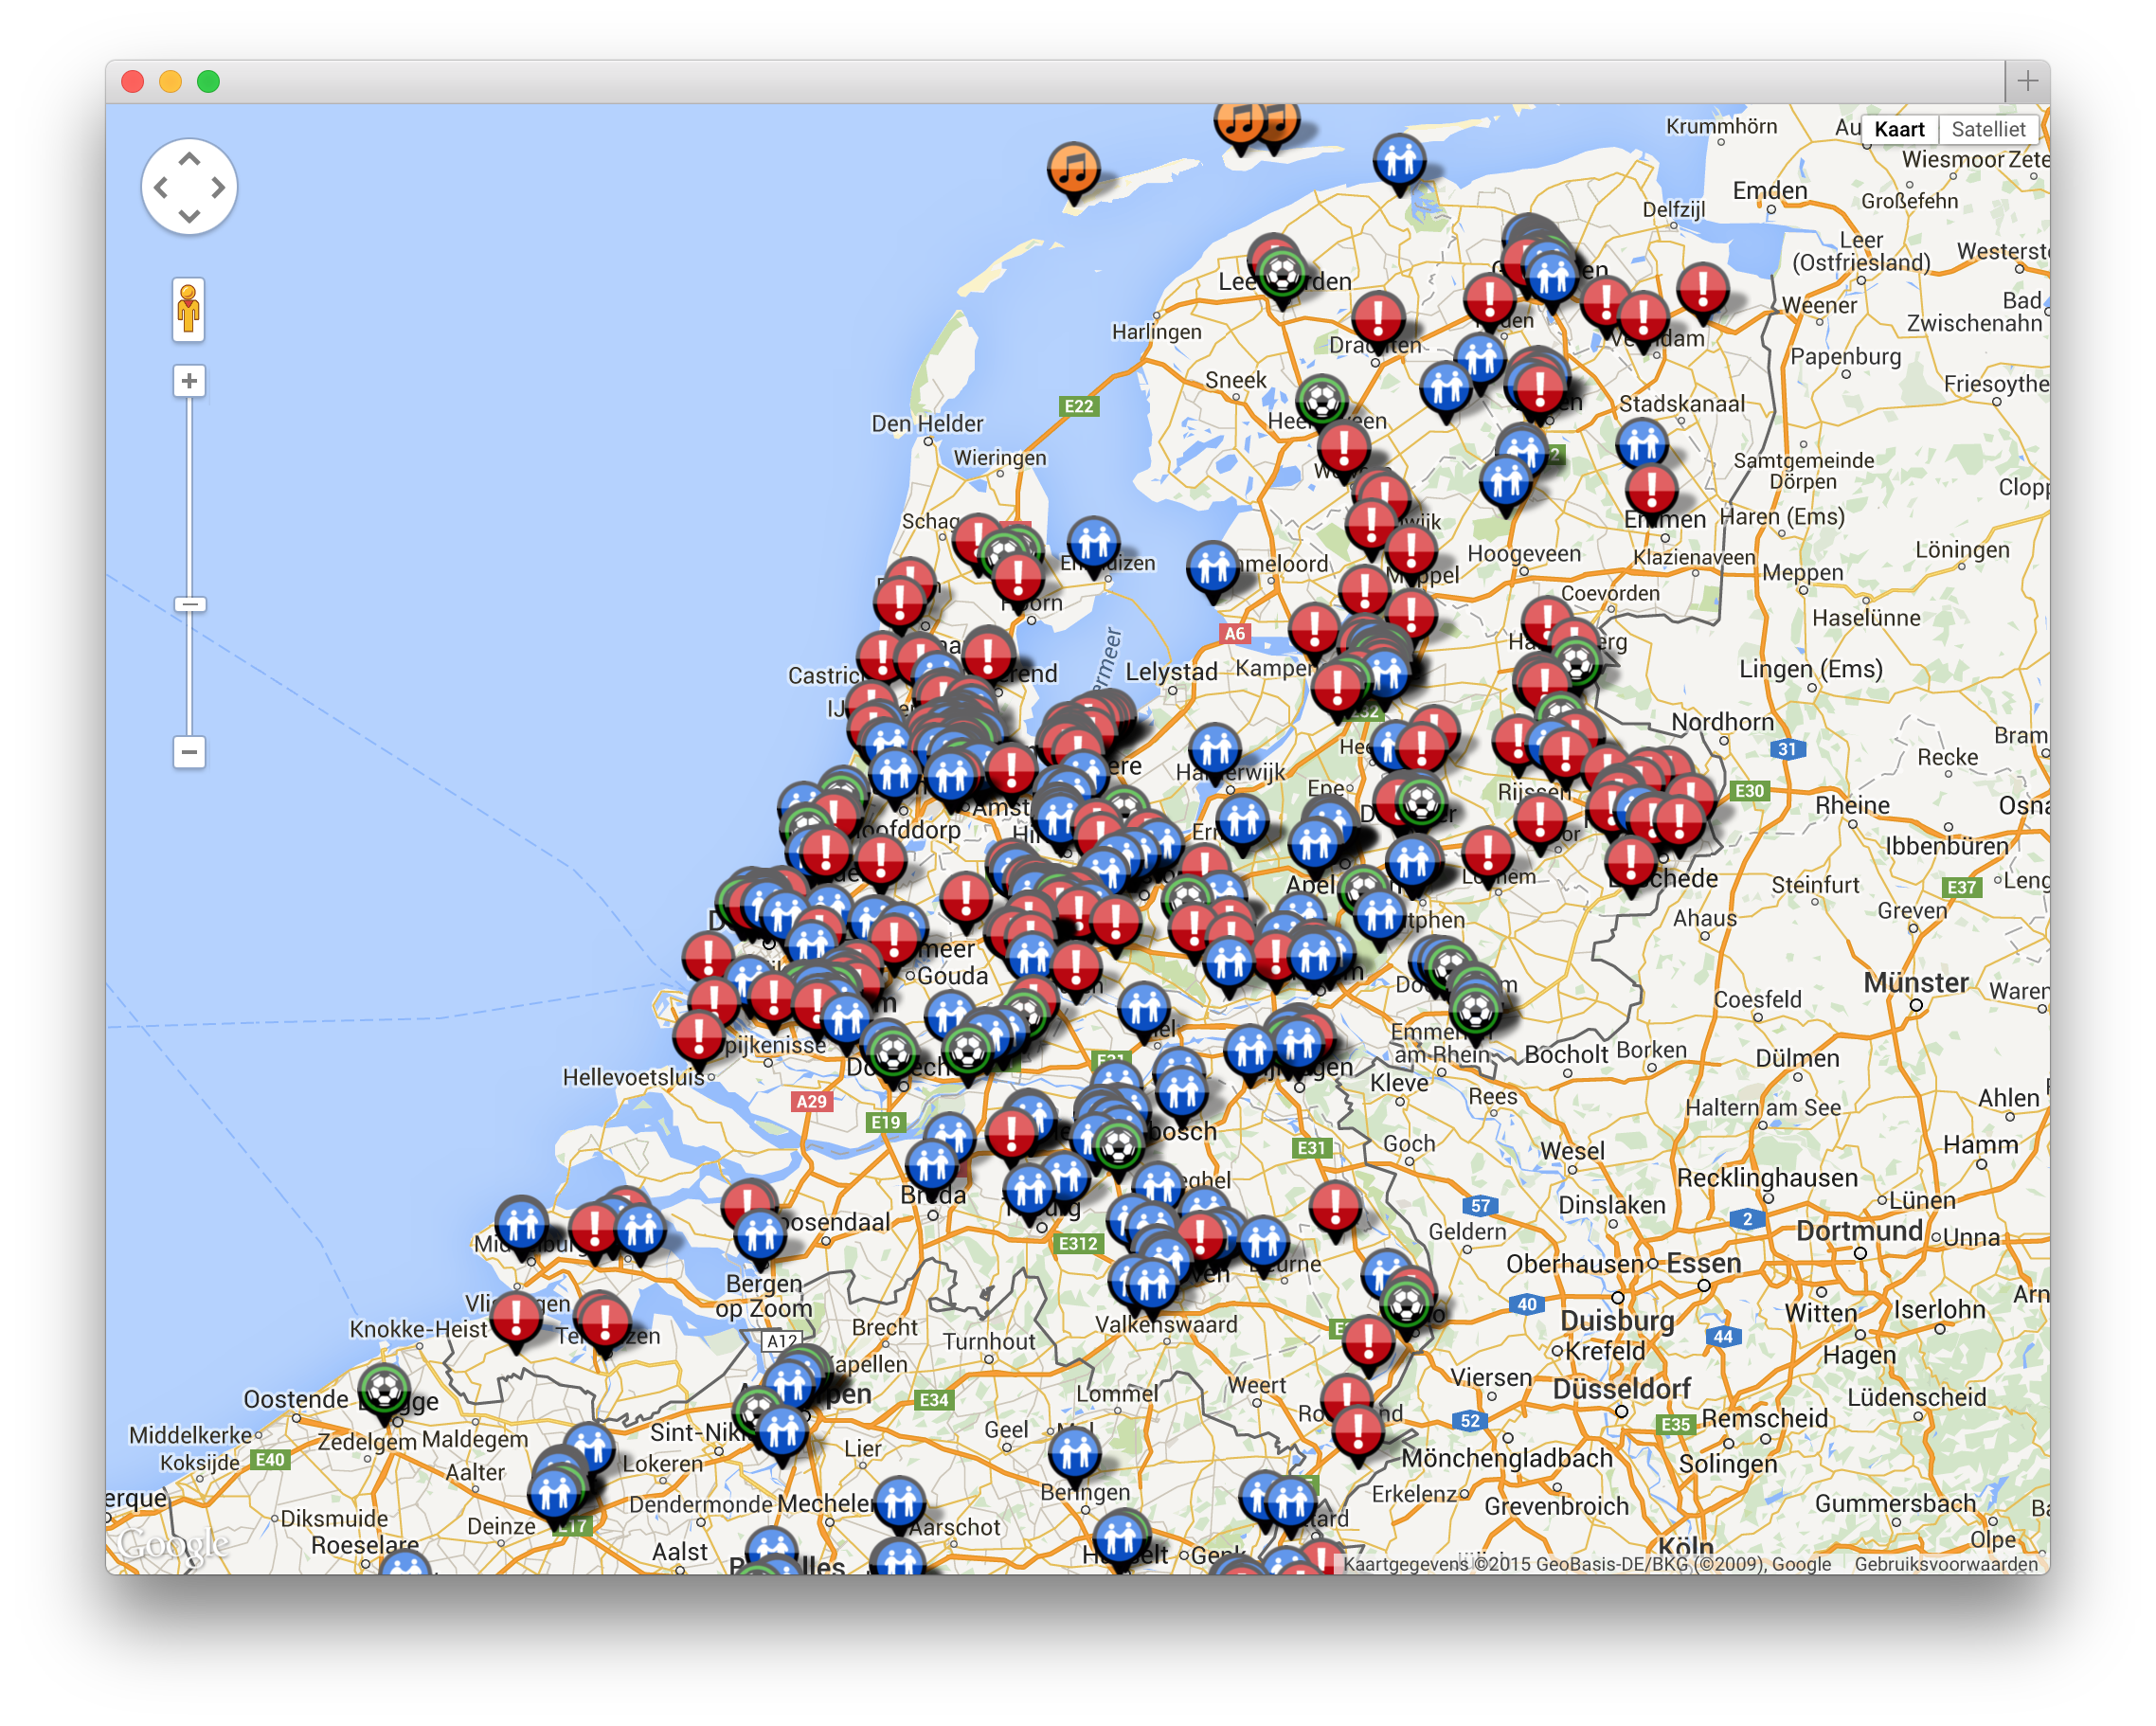
\includegraphics[width=4.5in]{voorkant.png} 
   \caption{GUI}
   \label{fig:gui}
\end{figure}
\clearpage


\setcounter{tocdepth}{2} % Set the depth of the table of contents to show sections and subsections only
\tableofcontents % Print the table of contents

%\listoffigures % Print the list of figures

%\listoftables % Print the list of tables

%----------------------------------------------------------------------------------------
%	ABSTRACT
%----------------------------------------------------------------------------------------
\clearpage
\section*{Abstract} % This section will not appear in the table of contents due to the star (\section*)

\lipsum[1] % Dummy text


%----------------------------------------------------------------------------------------

\newpage % Start the article content on the second page, remove this if you have a longer abstract that goes onto the second page

%----------------------------------------------------------------------------------------
%	INTRODUCTION
%----------------------------------------------------------------------------------------

\section{Introduction}

%waarom
With the growing number of people using social media services like Twitter and the enormous amount of data available makes it interesting to use as a source of information about events that are taking place at a certain time and location. This real time information and with the addition about how people feel about these events can be very useful, for example to provide news items with more information about user sentiment.

%wat
This thesis describes a method of finding local events based on tweets with geo information and categorize them into 5 categories (No-event, Sport, Enterainment, Meeting, Incident) and to find relevant information within those tweets about the location and people involved. Local events are events that take place in a certain radius (\begin{math}Z\end{math}) within a certain time interval (\begin{math}X\end{math}). For this research \begin{math}z= 0.5km , x= 5 hours\end{math}.

My research question is: Is it possible to detect local events from the Twitter stream that take place in the Netherlands based on Tweets with geo-information, to see if you can detect what type of events take place and who the important people/organizations or topics are to make an interactive map of these events.

%hoe
You can read in the following chapters how the research was conducted

%----------------------------------------------------------------------------------------
%	Related literature
%----------------------------------------------------------------------------------------

\section{Related literature}
Walter and Kaisser[1] describe in their paper Geo-spatial event detection in the Twitter stream a way to recognize geo-spatial events. They focus on small events that take place in a small area like fires and traffic jams. It differs from my research because I want to focus on locations where events of different sizes can take place but the features they use can be useful for my research. Especially how they calculate the clusterscore (cluster of tweets from a region) can be useful. Unfortunately they do not describe how they make clusters of locations.

Amineh Amini et al.: Density-Based Data Streams Clustering Survey[2] is a paper about different clustering techniques and is interesting to see which ones I can use to make clusters of the locations and the events. DBSCAN is one of the density-based clustering algorithms I maybe can use.  DBSCAN (Density-Based Spatial Clustering of Applications with Noise) is developed for clustering large spatial databases with noise, based on connected regions with high density. The density of each point is defined based on the number of points close to that particular point called the point's neighborhood.
The dense neighborhood is defined based on two user-specified parameters: the radius (of the neighborhood, and the number of the objects in the neighborhood 




%----------------------------------------------------------------------------------------
%	METHOD
%----------------------------------------------------------------------------------------

\newpage
\section{Method}
In this chapter the used methods for the experiment are described. 

\subsection{Clustering}
The first task is to cluster the tweets based on their location and time. There are several approaches in location clustering that can be used. Because the aim of the research was to make something that could work in real-time it was necessary to look for an approach that was quick. GeoHash is is a system invented by Gustavo Niemeyer that converts latitude and longitude coordinates into a hash. The more digits used means a higher accuracy. If two locations share the same prefix indicates (not always) that the locations are nearby. This algorithm is quick and easy to use and ideal for my experiment.

Figure 2 illustrates that 1 digit can be used to represent a quarter of the world, two digits 1/16 and three digits 1/64 etc. 
\begin{figure}[htbp] %  figure placement: here, top, bottom, or page
   \centering
   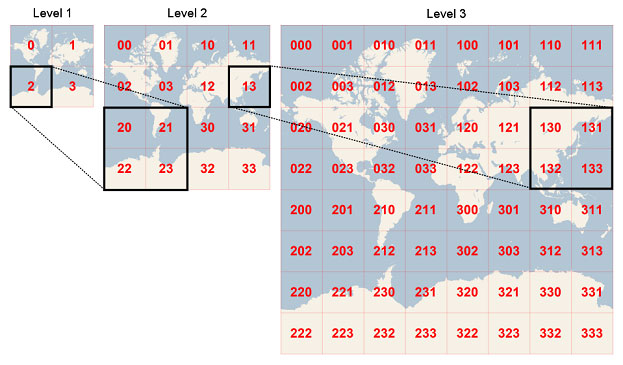
\includegraphics[width=4.5in]{geohash.jpg} 
   \caption{Geohash}
   \label{fig:geohash}
\end{figure}

There are several implementations of this algorithm in Python. I used the GeoHash library written in 2009 by Hiroaki Kawai because of the good documentation and excellent features. The function to calculate the GeoHash of a location requires the desired accuracy, latitude and longitude of that location and returns the GeoHash for that location. The library also provides functions to calculate the neighboring GeoHashes, this is useful because in a grid clustering approach border cases can occur and with this function neighboring GeoHashes can be explored to see if it contains tweets with the same topic and can merge them if necessary. 

\subsection{NLTK}
Python has a lot of functions to use while doing NLP tasks but for more advanced tasks it is not powerful enough. Therefore we have chosen the Natural Language Tookit (NLTK) %link naar bron.
NLTK has a lot of modules that can be used for a wide range of NLP tasks. It is also really easy to use and well documented. 

\subsection{Classification}
After forming the potential events (Event Candidates) the Event Candidates have to be classified as a specific event category or not an event.  NLTK provides excellent documentation and functions for classifying. \\\\  NLTK provides several classifier types:

\begin{itemize}[noitemsep]
\item ConditionalExponentialClassifier
\item DecisionTreeClassifier
\item MaxentClassifier
\item NaiveBayesClassifier
\item WekaClassifier
\end{itemize}

In the next chapter I describe the results using the different classifiers. Some classifiers where not used because they are used together with other software.


\subsection{Named Entity Reconinigzion}
For finding the important persons, organizations and locations i want to use Named Entity Reconinigzion(NER). NER is the proces of labeling data with corresponding categories like person, organization or location. For example:

\begin {quote}
Klaar voor Ajax (organization) - NAC(organization) @Amsterdam(location) @ArenAPoort(location) in Amsterdam(location) Zuidoost, Noord-Holland(location)
\end{quote}
Current NER tools were designed to process large texts and perform badly with tweets due to the noisy and short style. One of the most used NER tools is Stanford NER. This Java implementation is also known as CRFClassifier. The software comes with 3 trained classifiers that perform particularly well for the three classes persons, organizations and locations. Some experiments are done with using labeled tweets as traindata but mostly in English.  


%----------------------------------------------------------------------------------------
%	Experiment and Evaluation
%----------------------------------------------------------------------------------------
\newpage
\section{Experiment and Evaluation}
For my experiment I worked together with David de Kleer in collecting the data and building the Python modules. The goal was to build a system that can detect events that take place at a specific location, for example concerts, football matches, fires and traffic jams.  Events that take place on a larger scale like elections and extreme weather conditions are ignored. The input for this system are tweets that have coordinates that we afterwards try to cluster based on proximity, time and topic. These clusters of tweets are potential events that are system should classify as event/no event. The final goal was to plot these events on a map.
\subsection{System architecture}
Python was uded for this system because of the excellent tools available to build a machine learning system. NLTK and Scikit learn are used for classifying the event candidates.

We designed several classes for building our system but there are 3 main modules:

\begin{description}

\item[EventCandidates] 
The module that processes the tweets by giving each tweet a GeoHash, tokenizes the tweet and passes it through to the clusterCreator module that clusters the tweets using the geoHash and the timestamp resulting in event candidates. Finally the module clusterMerger checks for each event candidate if there are any neighboring event candidates that belong to each other and merges them. Finally the event candidates are saved as a datafile.


\item[Annotater] 
This module makes it possible for multiple judges to annotate the data created with the EventCandidates module. After finishing the annotation by both judges it calculates the Kappa score and other statistics and saves the annotation in a datafile.


\item[EventDetective] 
This module uses classification to detect events in the given event candidates and generates a Google map of events with corresponding category icons and wikified text.


\end{description}

\subsection{Data collection}
For the experiment tweets are used that have coordinates. Using a simple Grep command it was possible to retrieve only tweets with this information from the Karora machine. We collected two datasets. One set for testing and training and one for the final test (devset). 
The first dataset consisted of Dutch tweets from March 2015 that we have downloaded from the Karora machine. In total there where 566549 tweets with geo information. That is about 3procent of the total number of tweets published in that month. The Devset consists of 165848 tweets from the second half of April 2015.

\subsection{Annotation}
The data is annotated by two judges. The kappa score was 0.79 for the trainset and 0.8 for the devset. We defined the following categories:

\begin{itemize}[noitemsep] % [noitemsep] removes whitespace between the items for a compact look
\item \textbf{Other (OTH)} All events that are other then the following categories 
\item \textbf{Meeting (MEE)} All events that are meetings or conferences 
\item \textbf{Entertainment (ENT)} All events that have to do with concerts, movies or theater
\item \textbf{No Event (NOE)} No Event
\item \textbf{Sport (SPO)} All events that have to do with sport 
\end{itemize}
For the testset we annotated 1350 event candidates with these categories. In 87\% of the cases the judges agreed.

\begin{table}[h]
\begin{tabular}{lcccccc}
 & \multicolumn{1}{l}{\textbf{OTH}} & \multicolumn{1}{l}{\textbf{MEE}} & \multicolumn{1}{l}{\textbf{ENT}} & \multicolumn{1}{l}{\textbf{NOE}} & \multicolumn{1}{l}{\textbf{INC}} & \multicolumn{1}{l}{\textbf{SPO}} \\ \cline{2-7} 
\multicolumn{1}{l|}{\textbf{OTH}} & \multicolumn{1}{c|}{\textless1\textgreater} & \multicolumn{1}{c|}{.} & \multicolumn{1}{c|}{.} & \multicolumn{1}{c|}{2} & \multicolumn{1}{c|}{1} & \multicolumn{1}{c|}{1} \\ \cline{2-7} 
\multicolumn{1}{l|}{\textbf{MEE}} & \multicolumn{1}{c|}{21} & \multicolumn{1}{c|}{\textless207\textgreater} & \multicolumn{1}{c|}{7} & \multicolumn{1}{c|}{25} & \multicolumn{1}{c|}{.} & \multicolumn{1}{c|}{2} \\ \cline{2-7} 
\multicolumn{1}{l|}{\textbf{ENT}} & \multicolumn{1}{c|}{3} & \multicolumn{1}{c|}{.} & \multicolumn{1}{c|}{\textless20\textgreater} & \multicolumn{1}{c|}{5} & \multicolumn{1}{c|}{.} & \multicolumn{1}{c|}{.} \\ \cline{2-7} 
\multicolumn{1}{l|}{\textbf{NOE}} & \multicolumn{1}{c|}{14} & \multicolumn{1}{c|}{27} & \multicolumn{1}{c|}{18} & \multicolumn{1}{c|}{\textless619\textgreater} & \multicolumn{1}{c|}{9} & \multicolumn{1}{c|}{9} \\ \cline{2-7} 
\multicolumn{1}{l|}{\textbf{INC}} & \multicolumn{1}{c|}{1} & \multicolumn{1}{c|}{2} & \multicolumn{1}{c|}{.} & \multicolumn{1}{c|}{12} & \multicolumn{1}{c|}{\textless178\textgreater} & \multicolumn{1}{c|}{.} \\ \cline{2-7} 
\multicolumn{1}{l|}{\textbf{SPO}} & \multicolumn{1}{c|}{1} & \multicolumn{1}{c|}{.} & \multicolumn{1}{c|}{.} & \multicolumn{1}{c|}{5} & \multicolumn{1}{c|}{.} & \multicolumn{1}{c|}{60\textgreater} \\ \cline{2-7} 
\end{tabular}
\caption[Table caption text]{Confusion matrix testset annotation }
\end{table}

For the devset we annotated 500 event candidates with these categories. In 86\% of the cases the judges agreed.

\begin{table}[h]
\begin{tabular}{lcccccc}
                                  & \multicolumn{1}{l}{\textbf{OTH}}            & \multicolumn{1}{l}{\textbf{MEE}}              & \multicolumn{1}{l}{\textbf{ENT}}            & \multicolumn{1}{l}{\textbf{NOE}}              & \multicolumn{1}{l}{\textbf{INC}}             & \multicolumn{1}{l}{\textbf{SPO}}    \\ \cline{2-7} 
\multicolumn{1}{l|}{\textbf{OTH}} & \multicolumn{1}{c|}{\textless.\textgreater} & \multicolumn{1}{c|}{.}                        & \multicolumn{1}{c|}{.}                      & \multicolumn{1}{c|}{.}                        & \multicolumn{1}{c|}{1}                       & \multicolumn{1}{c|}{.}              \\ \cline{2-7} 
\multicolumn{1}{l|}{\textbf{MEE}} & \multicolumn{1}{c|}{4}                      & \multicolumn{1}{c|}{\textless110\textgreater} & \multicolumn{1}{c|}{13}                     & \multicolumn{1}{c|}{9}                        & \multicolumn{1}{c|}{.}                       & \multicolumn{1}{c|}{3}              \\ \cline{2-7} 
\multicolumn{1}{l|}{\textbf{ENT}} & \multicolumn{1}{c|}{.}                      & \multicolumn{1}{c|}{.}                        & \multicolumn{1}{c|}{\textless8\textgreater} & \multicolumn{1}{c|}{2}                        & \multicolumn{1}{c|}{.}                       & \multicolumn{1}{c|}{.}              \\ \cline{2-7} 
\multicolumn{1}{l|}{\textbf{NOE}} & \multicolumn{1}{c|}{3}                      & \multicolumn{1}{c|}{19}                       & \multicolumn{1}{c|}{4}                      & \multicolumn{1}{c|}{\textless199\textgreater} & \multicolumn{1}{c|}{4}                       & \multicolumn{1}{c|}{2}              \\ \cline{2-7} 
\multicolumn{1}{l|}{\textbf{INC}} & \multicolumn{1}{c|}{1}                      & \multicolumn{1}{c|}{.}                        & \multicolumn{1}{c|}{.}                      & \multicolumn{1}{c|}{.}                        & \multicolumn{1}{c|}{\textless78\textgreater} & \multicolumn{1}{c|}{.}              \\ \cline{2-7} 
\multicolumn{1}{l|}{\textbf{SPO}} & \multicolumn{1}{c|}{.}                      & \multicolumn{1}{c|}{1}                        & \multicolumn{1}{c|}{2}                      & \multicolumn{1}{c|}{2}                        & \multicolumn{1}{c|}{.}                       & \multicolumn{1}{c|}{60\textgreater} \\ \cline{2-7} 
\end{tabular}
\caption[Table caption text]{Confusion matrix devset annotation }
\end{table}


\subsection{Creating Event Candidates}
We first processed all tweets by giving each tweet a GeoHash (see chapter x) and tokenize the tweet. That resulted in a dictionary of tweets that we used in the second step, clustering the tweets. The clusterCreator merged all GeoHashes and added the tweets to the correct time period using the function below :
\begin{python}

#setting used for this experiment
self.MINUTES = 60

def __createClusters(self):
        for tweet in self.tweetDicts:
            geoHash = tweet["geoHash"]
            tweetTime = tweet["unixTime"]
            foundTime = tweetTime

            if geoHash in self.clusters:
                for times in self.clusters[geoHash].keys():
                    if times <= tweetTime <= times + self.MINUTES * 60:
                        foundTime = times
            
            self.clusters[geoHash][foundTime].append(tweet)
            if tweetTime != foundTime:
                # use new timestamp as key to keep event active
                self.clusters[geoHash][tweetTime] = self.clusters[geoHash][foundTime]
                # Remove old key
                del self.clusters[geoHash][foundTime] 
\end{python}
The result is a dataset with potential events that we call Event Candidates.

With the use of GeoHash it is possible to have cases where the event is on a border resulting in two events which is actually is one event. We used the module clusterMerger to merge those clusters. This module iterates through all Event Candidates and calculates its neighbors GeoHashes. It then iterates over all neighbors if there are events in the same period. It also checks if the overlap in words is high enough, if so the clusters are merged. 


\subsection{Event detection}
\lipsum[10]

\subsubsection{Feature selection}
\lipsum[12]

\subsection{Named Entity Recognizion}
Because the available classifiers in the Stanford NER are not suitable for Tweets i trained my own classifier. First i collected a list of Dutch words of each category (Location, Persons, Organizations and Miscellaneous) I used the wordlist of Alpino,  software that is developed by Professor Gert-jan van Noord. Then i collected one million tweets that have at least one of the words. The second step was to automatically annotate the tweets. I wrote a Python script that processes each tweet and assigns the correct class based on the wordlists to each token and creates the training file. The training file was split to make a testfile (4/5 for the training and 1/5 for testing)


\newpage
\subsection{Results}



\subsubsection{Classifier}
\begin{table}[h]
\begin{tabular}{l|l|l|l|l|l|l|l|l|l|}
\cline{2-10}
                          & \multicolumn{3}{c|}{Naive Bayes}                                         & \multicolumn{3}{c|}{Maximum Entropy}                                     & \multicolumn{3}{c|}{SVM}             \\ \cline{2-10} 
                          & \multicolumn{3}{c|}{Accuracy = 84\%}                                     & \multicolumn{3}{c|}{Accuracy = 83\%}                                     & \multicolumn{3}{c|}{Accuracy = 81\%} \\ \cline{2-10} 
                          & \multicolumn{1}{c|}{P} & \multicolumn{1}{c|}{R} & \multicolumn{1}{c|}{F} & \multicolumn{1}{c|}{P} & \multicolumn{1}{c|}{R} & \multicolumn{1}{c|}{F} & P          & R          & F          \\ \hline
\multicolumn{1}{|l|}{NOE} & 0.85                   & 0.90                   & 0.88                   & 0.83                   & 0.93                   & 0.88                   & 0.85       & 0.83       & 0.84       \\ \hline
\multicolumn{1}{|l|}{SPO} & 0.77                   & 0.49                   & 0.60                   & 0.77                   & 0.49                   & 0.60                   & 0.77       & 0.49       & 0.60       \\ \hline
\multicolumn{1}{|l|}{ENT} & 0.00                   & 0.00                   & 0.00                   & 0.00                   & 0.00                   & 0.00                   & 0.00       & 0.00       & 0.00       \\ \hline
\multicolumn{1}{|l|}{MEE} & 0.76                   & 0.79                   & 0.77                   & 0.79                   & 0.74                   & 0.76                   & 0.65       & 0.81       & 0.72       \\ \hline
\multicolumn{1}{|l|}{INC} & 0.97                   & 0.97                   & 0.97                   & 0.94                   & 0.94                   & 0.94                   & 1.00       & 0.97       & 0.99       \\ \hline
\multicolumn{1}{|l|}{OTH} & 0.00                   & 0.00                   & 0.00                   & 0.00                   & 0.00                   & 0.00                   & 0.00       & 0.00       & 0.00       \\ \hline
\end{tabular}
\caption[Table caption text]{Results using all features }
\end{table}


\begin{table}[h]
\begin{tabular}{|l|c|c|c|c|c|c|}
\hline
    & \multicolumn{1}{l|}{OTH} & \multicolumn{1}{l|}{MEE} & \multicolumn{1}{l|}{ENT} & \multicolumn{1}{l|}{NOE} & \multicolumn{1}{l|}{INC} & \multicolumn{1}{l|}{SPO} \\ \hline
OTH & \textless.\textgreater   & .                        & .                        & 1.                       & .                        & .                        \\ \hline
MEE & .                        & \textless82\textgreater  & 2                        & 14                       & .                        & 12                       \\ \hline
ENT & .                        & .                        & \textless.\textgreater   & 1                        & .                        & .                        \\ \hline
NOE & .                        & 27                       & 5                        & \textless179\textgreater & 1                        & 7                        \\ \hline
INC & .                        & .                        & .                        & 2                        & \textless76\textgreater  & .                        \\ \hline
SPO & .                        & 1                        & 1                        & 2                        & 1                        & \textless16\textgreater  \\ \hline
\end{tabular}

\caption[Table caption text]{Confusion Matrix Naive Bayes }
\end{table}

\begin{table}[h]
\begin{tabular}{|l|c|c|c|c|c|c|}
\hline
    & \multicolumn{1}{l|}{OTH} & \multicolumn{1}{l|}{MEE} & \multicolumn{1}{l|}{ENT} & \multicolumn{1}{l|}{NOE} & \multicolumn{1}{l|}{INC} & \multicolumn{1}{l|}{SPO} \\ \hline
OTH & \textless.\textgreater   & 1                        & .                        & .                        & .                        & .                        \\ \hline
MEE & .                        & \textless81\textgreater  & 2                        & 7                        & 2                        & 11                       \\ \hline
ENT & .                        & .                        & \textless.\textgreater   & .                        & 1                        & .                        \\ \hline
NOE & .                        & 26                       & 5                        & \textless186\textgreater & 1                        & 7                        \\ \hline
INC & .                        & 1                        & .                        & 4                        & \textless73\textgreater  & .                        \\ \hline
SPO & .                        & 1                        & 1                        & 2                        & 1                        & \textless16\textgreater  \\ \hline
\end{tabular}
\caption[Table caption text]{Confusion Matrix Maximum Entropy }
\end{table}

\begin{table}[h]
\begin{tabular}{|l|c|c|c|c|c|c|}
\hline
    & \multicolumn{1}{l|}{OTH} & \multicolumn{1}{l|}{MEE} & \multicolumn{1}{l|}{ENT} & \multicolumn{1}{l|}{NOE} & \multicolumn{1}{l|}{INC} & \multicolumn{1}{l|}{SPO} \\ \hline
OTH & \textless.\textgreater   & 1                        & .                        & .                        & .                        & .                        \\ \hline
MEE & .                        & \textless89\textgreater  & 2                        & 31                       &                          & 14                       \\ \hline
ENT & .                        & .                        & \textless.\textgreater   & .                        &                          & .                        \\ \hline
NOE & .                        & 19                       & 5                        & \textless166\textgreater & 1                        & 4                        \\ \hline
INC & .                        & .                        & .                        & .                        & \textless73\textgreater  & .                        \\ \hline
SPO & .                        & 1                        & 1                        & 2                        & 1                        & \textless17\textgreater  \\ \hline
\end{tabular}
\caption[Table caption text]{SVM }
\end{table}




\subsubsection{NER}
I compare my results with the standard Stanford 4 class classifier. This classifier is trained on xxx and uses the same classes as my classifier.

\begin{table}[h]
\begin{tabular}{|l|l|l|l|l|l|l|}
\hline
Entity       & P      & R      & F1     & TP    & FP  & FN   \\ \hline
LOCATION     & 0,9623 & 0,9363 & 0,9491 & 4718  & 185 & 321  \\ \hline
MISC         & 0,9744 & 0,8964 & 0,9338 & 1903  & 50  & 220  \\ \hline
ORGANIZATION & 0,9711 & 0,9315 & 0,9509 & 4241  & 126 & 312  \\ \hline
PERSON       & 0,9031 & 0,8773 & 0,8900 & 4583  & 492 & 641  \\ \hline
Totals       & 0,9477 & 0,9118 & 0,9294 & 15445 & 853 & 1494 \\ \hline
\end{tabular}
\caption[Table caption text]{Classifier trained with Tweets }
\end{table}

\begin{table}[h]
\begin{tabular}{|l|l|l|l|l|l|l|}
\hline
Entity       & P      & R      & F1     & TP   & FP   & FN    \\ \hline
LOCATION     & 0,5779 & 0,2239 & 0,3227 & 1128 & 824  & 3911  \\ \hline
MISC         & 0,0280 & 0,0118 & 0,0166 & 25   & 869  & 2098  \\ \hline
ORGANIZATION & 0,2485 & 0,2554 & 0,2519 & 1163 & 3517 & 3390  \\ \hline
PERSON       & 0,2627 & 0,3084 & 0,2837 & 1611 & 4521 & 3613  \\ \hline
Totals       & 0,2875 & 0,2318 & 0,2567 & 3927 & 9731 & 13012 \\ \hline
\end{tabular}
\caption[Table caption text]{Stanford 4-class classifier }
\end{table}



\begin{landscape}
\begin{table}[h]
\begin{tabular}{|l|l|l|l|l|l|l|l|}
\hline
                          & accuracy & geen\_event    & sport          & entertainment  & bijeenkomst    & incident       & anders         \\ \hline
                          &          & P    R    F    & P    R    F    & P    R    F    & P    R    F    & P    R    F    & P    R    F    \\ \hline
All features              & 0.84     & 0.85 0.90 0.88 & 0.77 0.49 0.60 & 0.00 0.00 0.00 & 0.76 0.79 0.77 & 0.97 0.97 0.97 & 0.00 0.00 0.00 \\ \hline
Category                  & 0.81     & 0.85 0.82 0.84 & 0.73 0.46 0.56 & 0.00 0.00 0.00 & 0.66 0.84 0.74 & 0.99 0.97 0.98 & 0.00 0.00 0.00 \\ \hline
Location                  & 0.51     & 0.49 0.94 0.65 & 0.00 0.00 0.00 & 0.00 0.00 0.00 & 0.66 0.25 0.36 & 0.50 0.06 0.11 & 0.00 0.00 0.00 \\ \hline
WordOverlapSimple         & 0.63     & 0.60 0.85 0.71 & 0.00 0.00 0.00 & 0.00 0.00 0.00 & 0.57 0.33 0.42 & 0.77 0.83 0.80 & 0.00 0.00 0.00 \\ \hline
wordOverlapUser           & 0.6      & 0.57 0.93 0.71 & 0.00 0.00 0.00 & 0.00 0.00 0.00 & 0.00 0.00 0.00 & 0.66 0.90 0.76 & 0.00 0.00 0.00 \\ \hline
wordOverlapUser, category & 0.82     & 0.86 0.83 0.85 & 0.77 0.49 0.60 & 0.00 0.00 0.00 & 0.66 0.85 0.74 & 1.00 0.97 0.99 & 0.00 0.00 0.00 \\ \hline
\end{tabular}
\end{table}
\end{landscape}


%----------------------------------------------------------------------------------------

\end{document}